\section{Data Acquisition}

During data acquisition the subjects will be wearing the instruments presented earlier in \secref{methods:instrumentation}. The Shimmer3 devices will be placed, one on each leg, lateral distal to the knees of the subject.

The FSRs will be placed on the sole of each foot of the subject. One FSR 406 is placed at the lateral eminence of the sole. Of the two FSR 402 sensors, one will be placed under the heel and the other medial eminence of the sole. The Arduino-setup will be placed at the lower back of the subject and handle data collection. Collected data will be stored on an microSD card for offline analysis with MATLAB. An illustration of device placement on a subject can be seen in \figref{fig:bodySysSetup}.

%% SENSOR BAIT ALERT:
%jeg har skrevet at vi placere en FSR 406 (den store firkant sensor) under hælen. den skal sidde "bag" lilletåen.
%sensor bait tekst flyttet til bNEWSystemTest.tex

\begin{figure}[H]
	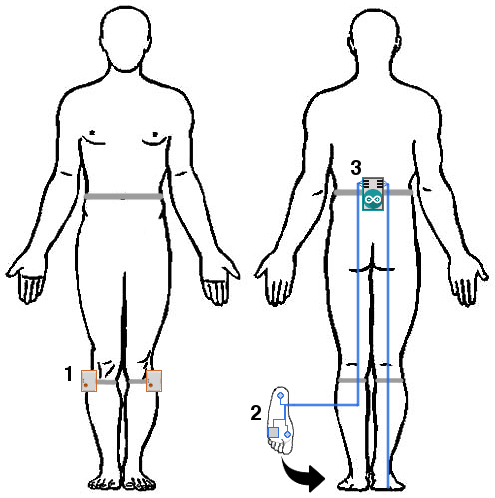
\includegraphics[width=.6\textwidth]{figures/bodySysSetup}
	\caption{The placement of the Shimmer3 IMU devices, Arduino-setup and FSRs on a test subject.}
	\label{fig:bodySysSetup}  %<--remember LABEL!
\end{figure}

Data acquisition from both the FSR sensors and the Shimmer3 devices are set to have a sample frequency of 100Hz. This sample rate is used by others performing similar measurements \cite{Verkerke2005, Byun2016, Sherwani2016}. Additionally, the sample rate is decided to be the same so it is possible to match the two data streams to each other, so it is possible to compare measured pressure forces under the feet while matching it to movement of the body. A simple graphical user interface (GUI) have been developed to match the data. This manual approach is favourable for this project as it were determined that it would be more time consuming to develop an algorithm to automatically match data streams. It would also go beyond the scope for the project.

Data from the Shimmer3 devices are send and saved directly to MATLAB via Bluetooth and stored in $nx3$ matrices, one for each leg.

For saving acquired data from the FSR sensors an Arduino program have been written to arrange measurements into an $nx6$ matrix. Each column corresponds with the channel input for each FSR. See \figref{fig:FSRNumbering} for the numbering of FSRs and channels. Rows in the matrix are time steps. The data is saved to a $.txt$-file on the microSD card. 

\begin{figure}[H]
	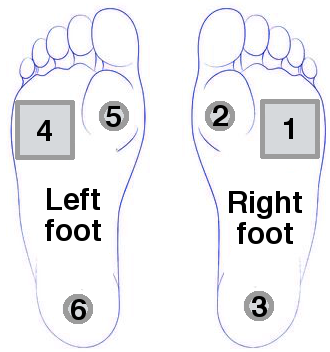
\includegraphics[width=.6\textwidth]{figures/FSRNumbering}
	\caption{The numbering of each FSR sensor according to the channel they are recorded to in the Arduino program.}
	\label{fig:FSRNumbering}  %<--remember LABEL!
\end{figure}

maybe something on filtering if we end up doing that

MATLAB alignment GUI description

MATLAB COP code description





All data is collected in MATLAB and organized into matrices. then something happens about calculating center of balance and maybe some rotational speed and something. 

Data acquisition from the Shimmer devices are handled by Bluetooth between the Shimmer devices and MATLAB. Sample frequency over 9000. Data is organized into a matrix, because that is the smart thing to do, when doing things in MATLAB.



so far there might not be any filtering of any of the data


